\chapter{Codes}
\begin{wrapfigure}[7]{l}{0.2\textwidth}
 \vspace{-28pt}
 \begin{center}
    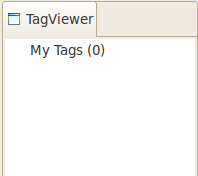
\includegraphics[width=0.18\textwidth]{img/codebrowser}
  \end{center}
  \vspace{12pt}
\end{wrapfigure}
Mit FreeQDA können Passagen aus Texten mit beliebigen Codes (auch \textit{Tag} genannt) markiert werden. Sind alle Texte mit den %
gewünschten Codes versehen, kann FreeQDA für beliebige Codes eine Übersichtsseite erzeugen, auf welcher jene Textstellen aufgelistet werden, die %
mit dem jeweiligen Code markiert wurden. 
Ähnlich wie bei Texten können Codes beliebig in Kategorien sortiert werden. Hierfür steht in der Navigationsleiste der \texttt{TagViewer} %
bereit. Innerhalb des TagViewers werden alle Code-Kategorien und Codes aufgelistet. Wenn Sie ein neues Projekt beginnen, ist diese Liste %
natürlich zunächst leer. 


\section{Einen neuen Code erstellen}
Neue Codes werden ähnlich angelegt wie Texte. Wählen Sie aus dem Programm-Menü den Punkt \texttt{Codes => Create Tag} aus (Abbildung \ref{fig:newtag1}). %
Alternativ können Sie auch %
die Maus über den TagViewer führen und die rechte Maustaste klicken. Es öffnet sich ein neues Fenster, in welchem Sie aufgefordert werden den %
Namen des neuen Codes einzutragen (Abbildung \ref{fig:tagname}). Tragen Sie also den Namen ein und klicken Sie anschließend auf das kleine %
Kästchen neben \texttt{Color}.

\begin{figure}[!hb]
\begin{minipage}[!hb!]{0.5\textwidth}
	\centering
	 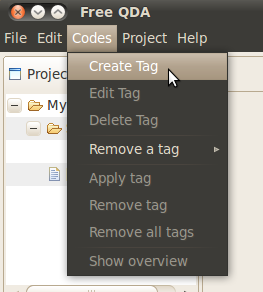
\includegraphics[width=0.42\textwidth]{img/createtag1}
	\caption{Tag erstellen}
	\label{fig:newtag1}
\end{minipage}
\hfill
\begin{minipage}[!hb!]{0.5\textwidth}
	\centering
	 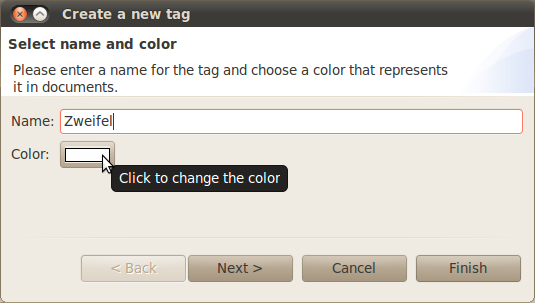
\includegraphics[width=0.8\textwidth]{img/tagname}
	\caption{Name des Tags}
	\label{fig:tagname}
\end{minipage}
\end{figure}

Es öffnet sich nun ein weiteres Fenster, in welchem Sie die gewünschte Code-Farbe auswählen können (Abbildung \ref{fig:tagfarbe1}). %
Mit der Farbe, die Sie hier auswählen, werden die Textstellen, die mit dem Code getaggt werden, farblich hinterlegt. Haben Sie eine Farbe %
gewählt, bestätigen Sie Ihre Auswahl durch Klick auf \texttt{OK}. Die ausgewählte Farbe wird nun auch im Namensfenster des neuen Tags %
angezeigt (Abbildung \ref{fig:tagfarbe2}). Klicken Sie nun auf \texttt{Finish} um den Code zu erzeugen.

\begin{figure}[!hb]
\begin{minipage}[!hb!]{0.5\textwidth}
	\centering
	 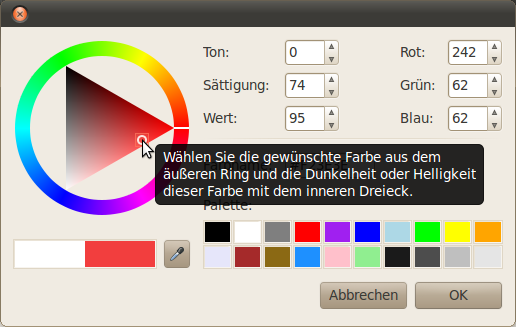
\includegraphics[width=0.5\textwidth]{img/tagfarbe}
	\caption{Tagfarbe auswählen}
	\label{fig:tagfarbe1}
\end{minipage}
\hfill
\begin{minipage}[!hb!]{0.5\textwidth}
	\centering
	 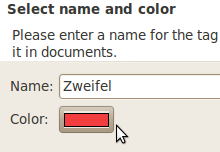
\includegraphics[width=0.45\textwidth]{img/tagfarbe2}
	\caption{Tagfarbe}
	\label{fig:tagfarbe2}
\end{minipage}
\end{figure}

\section{Einen Code unterhalb eines anderen Codes erstellen}
\begin{wrapfigure}[11]{l}{0.5\textwidth}
 \vspace{-28pt}
 \begin{center}
    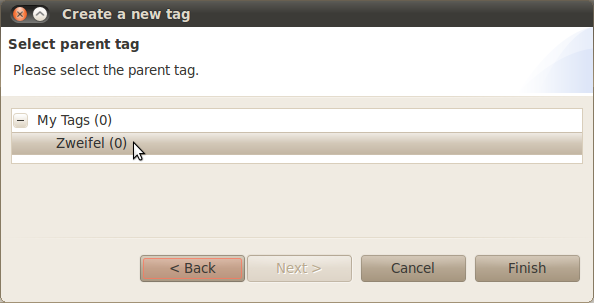
\includegraphics[width=0.48\textwidth]{img/subtag}
	\caption{Tag-Kategorie wählen}
	\label{fig:subtag}
  \end{center}
  \vspace{12pt}
\end{wrapfigure}
Ähnlich wie bei Textkategorien (siehe Seite \pageref{sec:textcategory}), können auch Codes ineinader verschachtelt werden. 
Legen Sie zunächst wie oben beschrieben einen neuen Tag an, indem Sie in der Menüleiste auf \texttt{Codes => Create Tag} klicken. %
Es öffnet sich das Fenster, in welchem Sie den Tagnamen sowie die Farbe auswählen können. Klicken Sie hier auf den \texttt{Next}-Button %
(und \textbf{nicht} auf \texttt{Finish}). Es wird Ihnen nun eine Liste aller vorhandenen Codes angezeigt. Klicken Sie hier auf den %
Code, unterhalb welchen der neue Code angelegt werden soll (Abbildung \ref{fig:subtag}). Bestätigen Sie Ihre Auswahl per %
Klick auf \texttt{Finish}.\\[4mm] %

\begin{wrapfigure}[3]{l}{0.2\textwidth}
 \vspace{-28pt}
 \begin{center}
    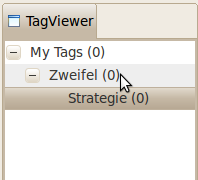
\includegraphics[width=0.18\textwidth]{img/tagviewer}
  \end{center}
  \vspace{12pt}
\end{wrapfigure}

Der neue Code wird nun im TagViewer angezeigt und kann von dort ausgewählt und verwendet werden. In unserem Beispiel wurde der %
Code \textit{Strategie} unterhalb des Codes \textit{Zweifel} angelegt.\\[16mm]
\vfill
\section{Eine Textstelle taggen}
\begin{wrapfigure}[9]{l}{0.4\textwidth}
 \vspace{-28pt}
 \begin{center}
    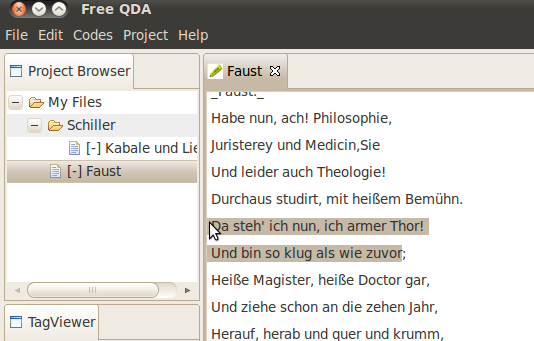
\includegraphics[width=0.38\textwidth]{img/tagtext1}
	\caption{Textstelle markieren}
	\label{fig:texttag1}
  \end{center}
  \vspace{12pt}
\end{wrapfigure}

Eine der Hauptaufgaben von FreeQDA ist es, Textstellen mit beliebigen Codes zu taggen. Um eine Textstelle mit einem Code zu versehen öffnen %
Sie zunächst den gewünschten Text im FreeQDA-Editor. Hierzu führen Sie im Project Browser einen Doppelklick auf den gewünschten Text aus. %
Suchen Sie nun innerhalb des Editors eine passende Textstelle aus, die Sie mit einem Code versehen möchten. Markieren Sie diesen %
Textbereich mit der Maus (siehe Abbildung \ref{fig:texttag1}).

\newpage

\begin{figure}[!hbt]
\begin{minipage}[!hb!]{0.5\textwidth}\scriptsize
	\centering
	 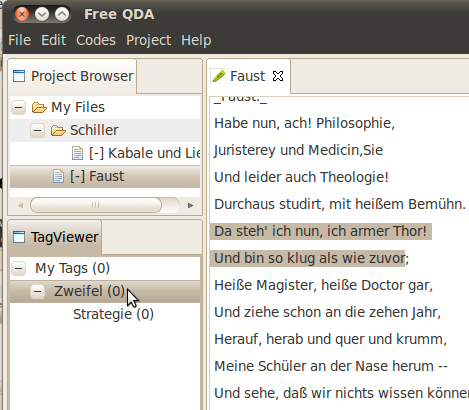
\includegraphics[width=0.7\textwidth]{img/tagtext2}
	\caption{Tag auswählen}
	\label{fig:texttag2}
\end{minipage}
\hfill
\begin{minipage}[!hb!]{0.5\textwidth}
	\centering
	 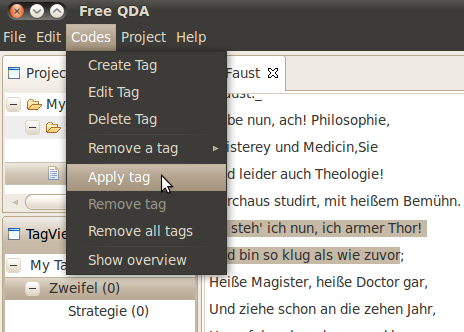
\includegraphics[width=0.8\textwidth]{img/tagtext3}
	\caption{Code setzen}
	\label{fig:texttag3}
\end{minipage}
\end{figure}

Wählen Sie jetzt aus dem TagViewer den gewünschten Code aus (Abbildung \ref{fig:texttag2}). Anschließend wird der Code über den Menüpunkt %
\texttt{Codes => Apply tag} auf die Textstelle angewendet (Abbildung \ref{fig:texttag3}).  Alternativ können Sie auch mit der rechten Maustaste %
auf den gewünschten Code klicken. %
Innerhalb des Editors ist die Textstelle nun mit der Farbe des gesetzten %
Codes unterlegt (Abbildung \ref{fig:texttag4}). Wenn Sie innerhalb des Editors mit der Maus über eine getaggte Textstelle fahren und dort %
etwas warten, werden Ihnen weitere Informationen zu den gesetzten Codes angezeigt. Im Beispiel der Abbildung \ref{fig:texttag4} sehen Sie, %
dass die Textzeilen 843 bis 844 mit dem Code ``\textit{Zweifel}'' getaggt ist.


\begin{figure}[!hbt]
	\centering %\vspace{-26pt}
	 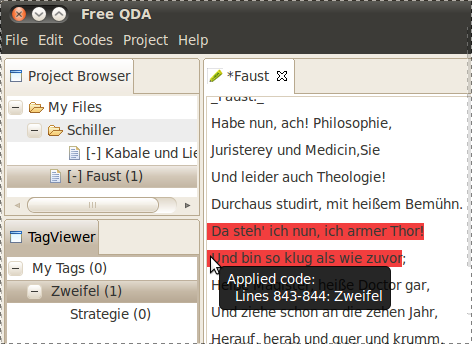
\includegraphics[width=0.5\textwidth]{img/tagtext4}
	\caption{Code im Text}
	\label{fig:texttag4}
\end{figure}

Des Weiteren können Sie sehen, dass in Abbildung \ref{fig:texttag4} sowohl hinter dem Text \textit{Faust} sowie hinter dem Code %
\textit{Zweifel} jeweils eine \texttt{1} angezeigt wird. Dies bedeutet, dass im Text \textit{Faust} insgesamt \textit{eine} kodierte %
Textstelle enthalten ist. Des Weiteren bedeutet es, dass der Code \texttt{Zweifel} insgesamt auf eine Textstelle angewendet wurde. 


\begin{wrapfigure}[4]{l}{0.3\textwidth}
 \vspace{-28pt}
 \begin{center}
    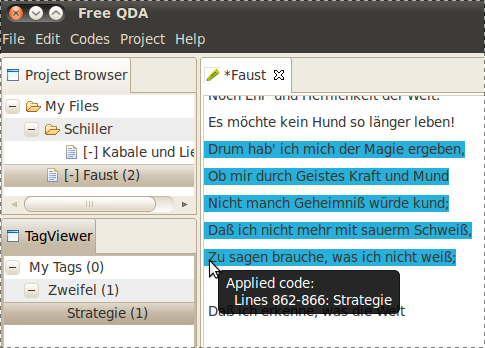
\includegraphics[width=0.28\textwidth]{img/tagtext5}
	\caption{Coden}
	\label{fig:texttag5}
  \end{center}
  \vspace{12pt}
\end{wrapfigure}

Wenn nun ein weitere Code gesetzt wird, erhöht sich die Zahl entsprechend. In Abbildung \ref{fig:texttag5} wurde eine weitere Textstelle des %
\textit{Faust} mit dem Code \textit{Strategie} getaggt. Dementsprechend erhöht sich der Zähler im Project Browser hinter \textit{Faust} %
auf 2.


\newpage
\section{Übersichten erstellen}
Haben Sie Textstellen mit Codes versehen, können Sie sich Übersichten für einzelne Codes in ausgewählten Texten anzeigen lassen. 
Hierfür ist es notwendig, die gewünschten Texte zunächst zu \textit{aktivieren}. Markieren Sie im Project Browser einen gewünschten Text. %
Wählen Sie anschließend aus dem Programm-Menü den Eintrag \texttt{Project => Activate text} (Abbildung \ref{fig:activatetext1}). %
Alternativ können Sie auch mit der rechten Maustaste auf den Text klicken. Einen aktivierten Text erkennen Sie an dem Symbol \texttt{[x]} %
vor dem Textnamen (siehe Mauszeiger in Abbildung \ref{fig:activatetext2}). Auf die selbe Weise können Sie Texte auch wieder de-aktivieren.

\begin{figure}[!hbt]
\begin{minipage}[!hb!]{0.5\textwidth}\scriptsize
	\centering
	 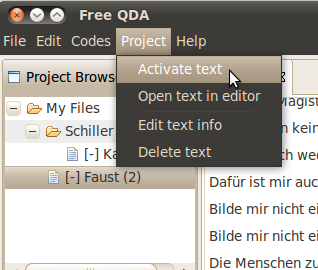
\includegraphics[width=0.7\textwidth]{img/activatetext1}
	\caption{Text aktivieren}
	\label{fig:activatetext1}
\end{minipage}
\hfill
\begin{minipage}[!hb!]{0.5\textwidth}
	\centering
	 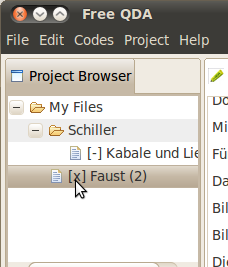
\includegraphics[width=0.5\textwidth]{img/activatetext2}
	\caption{aktivierter Text}
	\label{fig:activatetext2}
\end{minipage}
\end{figure}

Nachdem Sie alle gewünschten Texte aktiviert haben, markieren Sie im TagViewer einen Code, für welchen Sie eine Überischt erstellen möchten. %
Wählen Sie nun aus dem Programm-Menü den Eintrag \texttt{Codes => Show overview} (Abbildung \ref{fig:overview1}). Alternativ können Sie auch %
mit der rechten Maustaste auf den gewünschten Code klicken.

FreeQDA erzeugt nun eine Übersicht aller Textstellen in allen aktivierten Texten, die mit dem ausgewählten Code getaggt wurden (Abbildung \ref{fig:overview2}).
Da wir in unserem Beispiel den Code nur einmal vergeben haben, wird dementsprechend in Abbildung \ref{fig:overview2} auch nur diese eine %
Textstelle angezeigt.

Innerhalb der Überischt können Sie übrigens weitere Textstellen mit beliebigen Codes taggen. Ihre Eingaben werden in den Originaltexten gespeichert.
Natürlich können Sie die Übersichten auch ausdrucken. Wählen Sie hierzu im Programm-Menü den Punkt \texttt{File => Print}.

\begin{figure}[!hbt]
\begin{minipage}[!hb!]{0.5\textwidth}\scriptsize
	\centering
	 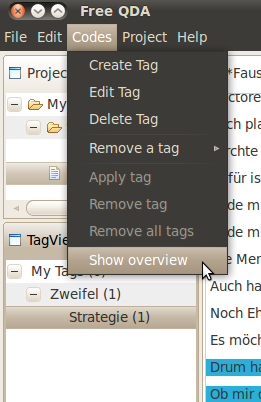
\includegraphics[width=0.4\textwidth]{img/showoverview}
	\caption{Übersicht erzeugen}
	\label{fig:overview1}
\end{minipage}
\hfill
\begin{minipage}[!hb!]{0.5\textwidth}
	\centering
	 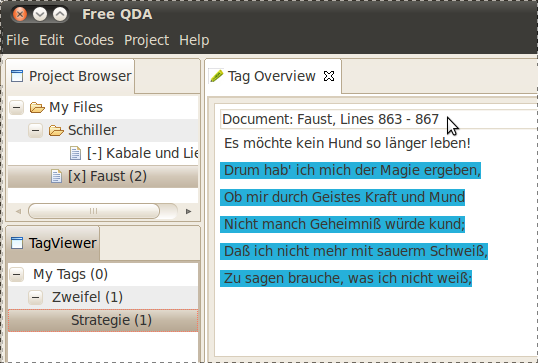
\includegraphics[width=0.9\textwidth]{img/overview1}
	\caption{Übersicht}
	\label{fig:overview2}
\end{minipage}
\end{figure}

